\chapter{Implementierung} \label{chap:implementierung}

Nachdem im letzten Kapitel (siehe \autoref{chap:Konzept}) das Konzept der Lösung der Aufgabenstellung beschrieben wurde, wird in diesem Kapitel die Implementierung der Software beschrieben.
Ziel ist es, alle beschriebenen Aufgabenteile in Python umzusetzen und eine Software zu entwickeln, die in der Lage ist, die Anforderungen der Aufgabenstellung zu erfüllen. Ausschnitte aus dieser Software sind im Kapitel des Konzepts bereits beschrieben und werden hier weiter ausgeführt.

Die Implementierung erfolgt in mehreren Schritten:

\begin{enumerate}
    \item \textbf{Umzug auf lokale Programmierung} 
    \item \textbf{Einpflegen der JSON-Parameter} 
    \item \textbf{Entwicklung der API} 
    \item \textbf{Installation im Labor}

\end{enumerate}

In den folgenden Kapiteln werden die einzelnen Schritte genauer beschrieben.

\section{Umzug auf lokale Programmierung} \label{subsec:umzug_auf_lokale_programmierung}

Die Struktur dieser Implementierung folgt der Konzeption der Programmstruktur nach dem MVC-Prinzip \autoref{fig:MVC_struktur}, welches in \autoref{sec:architektur} beschrieben ist.
Dieses Modell trennt die Datenverarbeitung, die Darstellung und die Steuerung der Software in drei verschiedene Module auf.
Die Datenverarbeitung wird in einem eigenen Modul abgetrennt, Darstellung und Steuerung sind in der API zusammengefasst.

Das Pycore-Modul, welches diese benötigten, selbst entwickelten Bibliotheken zur Verfügung stellt, ist auch in \autoref{fig:Projektstruktur} als eigener Ordner mit Python-Skripten in seinen Unterverzeichnissen dargestellt. Es beinhaltet die Funktionen, welche den Datensatz aufbereiten und dem neuronalen Netzwerk zum Training zur Verfügung stellen.
Die wichtigsten Bestandteile sind die Konvertierung in Graustufen, die Aufteilung des Datensatzes in Trainings- und Testdaten sowie der Download des untrainierten neuronalen Netzwerks und dessen Parametrisierung bezüglich der Klassifikationsaufgabe.

\begin{figure}[H]
    \centering
    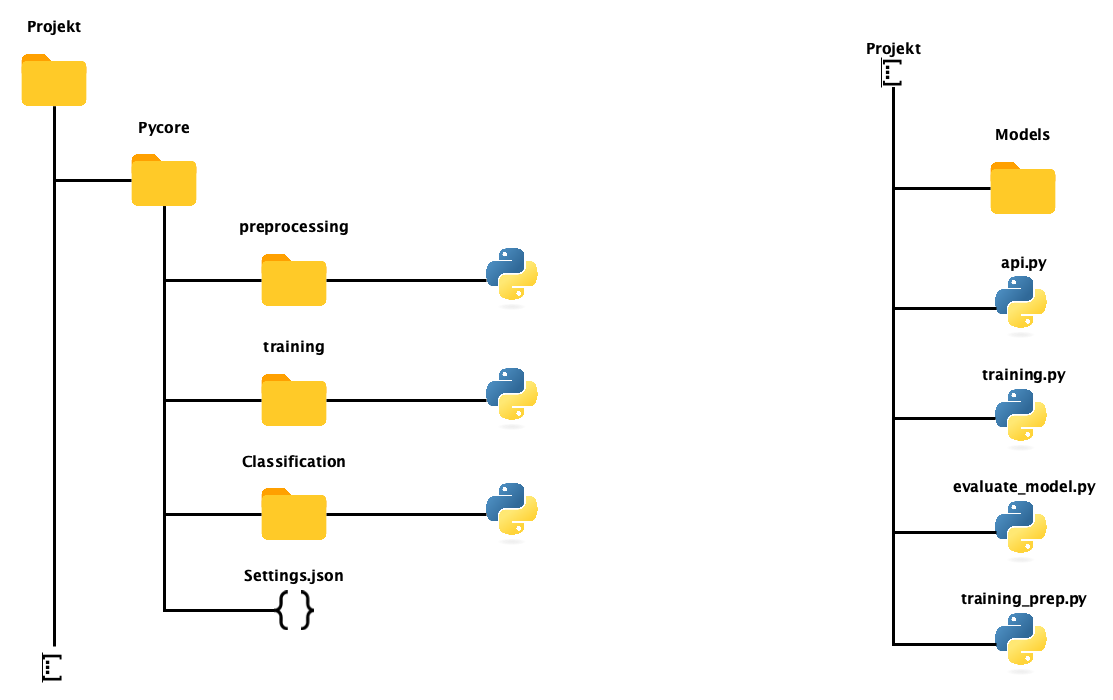
\includegraphics[width=0.8\textwidth]{Projektstruktur.png}
    \caption{Projektstruktur der Software im Dateiverzeichnis}
    \label{fig:Projektstruktur}
\end{figure}

Die in der Grafik \autoref{fig:Projektstruktur} dargestellte Dateistruktur repräsentiert ebenso die Struktur der Software. Die Funktionen werden in Bibliotheken im Pycore-Verzeichnis zusammengefasst. 
Sämtliche Daten werden in einem ausgegliederten Verzeichnis innerhalb des Projektverzeichnisses abgelegt. 

Im Projekthauptverzeichnis gibt es, neben des Pycore-Moduls und der Verzeichnisse für Trainings- und Testdaten, vier Python-Skripte. Diese können ausgeführt werden, um einzelne Teile der Software auszuführen.
\texttt{api.py} wird ausgeführt, um die Weboberfläche zu starten.
\texttt{train.py} wird ausgeführt, um das Modell zu trainieren.
\texttt{evaluate\_model.py} wird ausgeführt, um das Modell zu evaluieren und die in \autoref{sec:confusionmatrix} beschriebenen Werte zu erhalten. 
\texttt{training\_prep.py} kann ausgeführt werden, um den Datensatz zu verarbeiten, ohne das Modell zu trainieren.

Diese Skripte laden den jeweils benötigten Programmteil und die benötigten Parameter aus dem Pycore-Verzeichnis, führen die entsprechenden Funktionen aus und legen die Ergebnisse im Dateisystem ab.
Keines dieser Skripte ist über die Webanwendung zu erreichen, da sie nur für die interne Verwendung gedacht sind.

\section{Einpflegen der JSON-Parameter} \label{subsec:json_parameter}

Die Umsetzung des Konzeptes der Konfiguration der Programmparameter (siehe \autoref{sec:konfiguration}) erfolgt in Python mittels einer \ac{JSON}-Datei.
Diese Datei enthält alle Parameter, die für die Software benötigt werden.

\begin{lstlisting}[style=json, label=lst:json_example, caption={Beispiel einer \ac{JSON}-Datei mit Parametern des mobilnet Modells}]
    {
        "filepaths": {
            "good": "Bilder/Good_Pictures",
            "bad": "Bilder/Bad_Pictures",
            "good_gray": "Bilder/Good_Grayscale",
            "bad_gray": "Bilder/Bad_Grayscale",
            "train": "Bilder/train",
            "test":"Bilder/test",
            "validate":"Bilder/validate",
            "new": "Bilder/new"
        }
    }
\end{lstlisting}

Die Struktur der \ac{JSON}-Datei ist in \autoref{lst:json_example} dargestellt und wird in Python mittels des \texttt{json} Moduls eingelesen. Der hier dargestellte Ausschnitt beinhaltet alle wichtigen Dateipfade, um dem Python-Programm Zugriff zu den Trainings- und Testdaten sowie dem überwachten Ordner für neue Bilder zu gewähren. Er dient beispielhaft für das gesamte Programm. Ein Beispiel für das Einlesen der Datei ist in \autoref{lst:json_read} dargestellt.

\begin{lstlisting}[style=python, label=lst:json_read, caption={Einlesen der \ac{JSON}-Datei}]
    import json

    config_path = "pycore/setings.json"
    cf = json.load(open(config_path, 'r'))

    # Uebergabe der Parameter an die Funktionen
    uic.folder_to_grayscale(cf["filepaths"]["good"],cf["filepaths"]["good_gray"])
    uic.folder_to_grayscale(cf["filepaths"]["bad"],cf["filepaths"]["bad_gray"])

\end{lstlisting}

In diesem Codeausschnitt wird der Pfad zur Konfigurationsdatei festgelegt (Zeile 3) und die Datei wird eingelesen (Zeile 4). Die Parameter werden dann an die erste Funktion übergeben, welche die Bilder in Graustufen umwandelt und in einem separaten Verzeichnis ablegt (Zielverzeichnis siehe \autoref{lst:json_read}). Die Syntax für das Anwählen des Parameters ist \texttt{cf["filepaths"]["good"]}, wobei \texttt{cf} die Variable ist, in der die \ac{JSON}-Datei eingelesen wurde. Die \ac{JSON}-Datei wird als Array eingelesen, wobei der Zugriff auf die einzelnen Parameter über den Schlüssel in Textform erfolgt. In diesem Fall wird der Pfad zum Ordner mit den guten Bildern über den Schlüssel \texttt{"good"} angesprochen, während \texttt{"filepaths"} den Zugriff auf die passende Sektion des Arrays ermöglicht.

Angenommen der Benutzer wünscht ein anderes Verzeichnis für die Bilder, so kann er dies in der \ac{JSON}-Datei ändern und die Software erneut ausführen, ohne zu wissen, wo die Funktion, welche den Datensatz generiert, abliegt. 
Der gesamte Code dieses Projekts wurde nach diesem Schema aufgebaut, um eine einfache und einheitliche Konfiguration zu gewährleisten.

\section{Entwicklung der API} \label{subsec:entwicklung_der_api}

In diesem Abschnitt wird die Entwicklung der API beschrieben, welche die Kommunikation zwischen der Weboberfläche und der Backend-Logik der Software ermöglicht. 
Es wird sichergestellt, dass die Entwicklung dem Konzept der Aufgabenstellung \autoref{sec:weboberflaeche} entspricht.

Hierfür werden in zwei verschiedenen Threads zwei Funktionen ausgeführt werden. Die erste Funktion lädt das trainierte Modell in den Zwischenspeicher, um es für die Klassifizierung nutzbar zu machen (Zeile 3 \autoref{lst:api_exec}). Im zweiten Thread wird der Watchdog gestartet, welcher den Ordner für neue Bilder überwacht und bei neuen Bildern die Klassifizierung startet (Zeile 6). 


\begin{lstlisting}[style=python, label=lst:api_exec, caption={Start der Weboberfläche und der Threads in der api.py}]
    if __name__ == '__main__':

        model_thread = threading.Thread(target=load_model, daemon=True)
        model_thread.start()

        watchdog_thread = threading.Thread(target=start_watchdog, daemon=True)
        watchdog_thread.start()

        socketio.run(app, host="127.0.0.1", port=5000,debug=True,use_reloader=False)

\end{lstlisting}

Ziel des Threadings ist es, den Ordner für neue Bilder permanent zu überwachen, ohne zyklisch abzufragen. Dies spart Rechenleistung und ermöglicht eine schnellere Reaktion auf neue Bilder \cite{noauthor_threading_nodate}.

Parallel zu den beiden Threads wird die Weboberfläche in Zeile 9 des \autoref{lst:api_exec} gestartet. Bei Aufruf der Adresse, welche ebenfalls in Zeile 9 dargestellt ist, wird eine vorher definierte \ac{HTML}-Seite an den Browser des Clients mittels GET Anfrage (siehe \autoref{subsec:anfragearten_einer_api}) gesendet. 
Diese Seite enthält ein JavaScript, welches die Verbindung zum Websocket des Python-Programms herstellt und einen bidirektionalen Datenaustausch ermöglicht.

\begin{lstlisting}[style=html, label=lst:weboberflaeche, caption={JavaScript Code der Weboberfläche, welcher die Bilder des Websockets empfängt}]
        <script>
            var socket = io();
            socket.on('update_image', function(data) {
                console.log("Neues Bild-Event empfangen:", data);  // Debugging
                document.getElementById('latestImage').src = data.image_url + "?t=" + new Date().getTime();
            });
            socket.on('classification_result', function(data) {
            document.getElementById("classification-result").innerText = data.result;
            });
        </script>

\end{lstlisting}

Sobald ein neues Bild in den Ordner \texttt{Bilder/new} gelegt wird, wird ein Event ausgelöst, welches sowohl eine Klassifizierung herbeiführt als auch das Bild mittels Websocket an das JavaScript-Backend der Weboberfläche sendet. 

\section{Installation im Labor} \label{sec:installation}

Die Installation verläuft in drei Phasen: Übertragung, Installation und Tests.
Zunächst wird die Software auf einem \ac{USB}-Stick in das Labor gebracht und auf den Laborrechner kopiert. 
Der Laborrechner ist Teil des Lieferumfangs des FESTO \ac{cp-lab} Systems und steht dieser Studienarbeit zur Verfügung.

Dieser \Ac{PC} wird ausschließlich für die Steuerung der FESTO-Anlage verwendet und verwaltet die Datenbank, die Konfiguration der Stationen und die Programmierung der \ac{SPS}en. 
Python ist auf diesem Rechner bereits installiert, jedoch fehlen die benötigten Pakete für die Software. 
Alle benötigten Pakete werden in einem Python Virtual Environment installiert, um die Installation dieser Studienarbeit zu isolieren und die Funktionalität des bestehenden Systems nicht zu beeinträchtigen \cite{python_software_foundation_venv_nodate}.

Um eine Speicherung der von der Kamera aufgenommenen Bilder zu ermöglichen, muss innerhalb der Konfigurationssoftware der Kamera ein Archivierungspfad festgelegt werden. Dieser Pfad wird in der Software als Zielverzeichnis für die Klassifizierung genutzt. 

\begin{figure}[H]
    \centering
    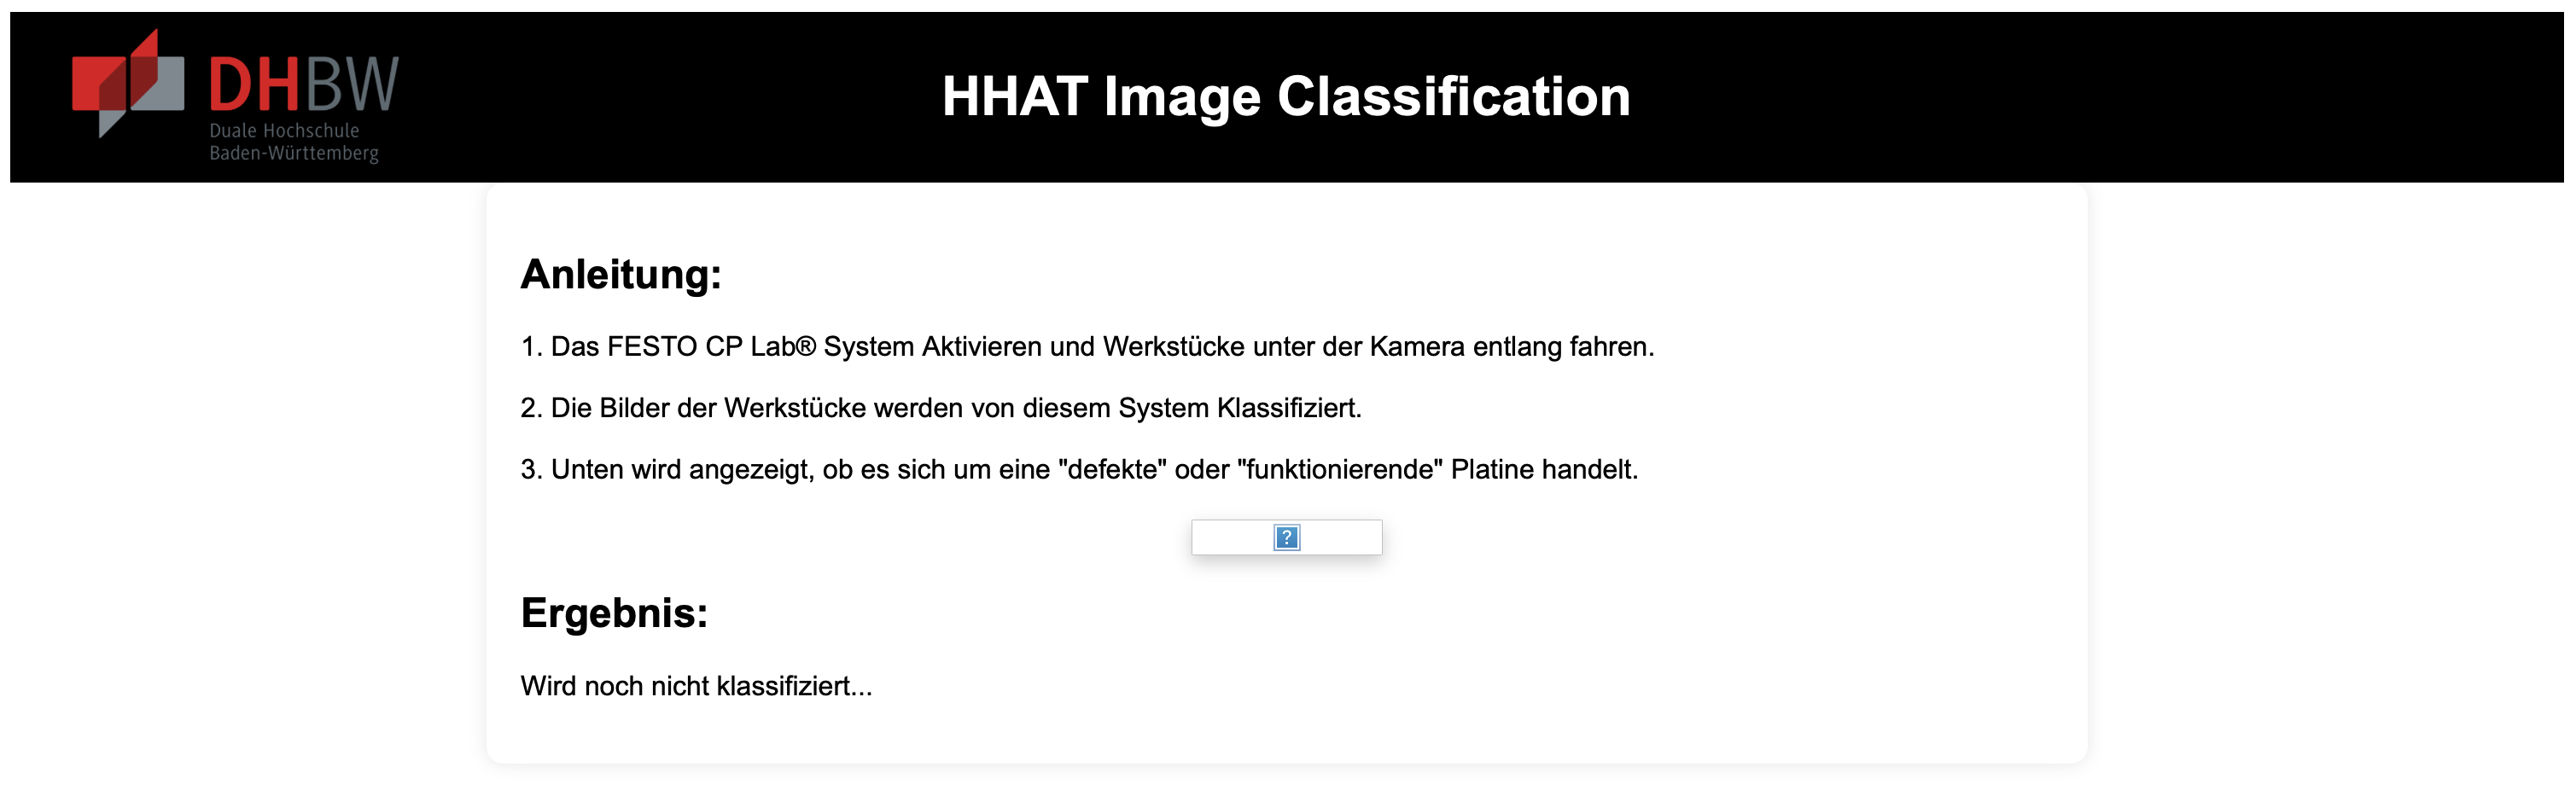
\includegraphics[width=1\textwidth]{Web-Ohne_Bild.png}
    \caption{Darstellung der Weboberfläche im Zustand ohne Klassifikation eines aktuellen \ac{PCB}s.}
    \label{fig:Weboverlay_teststadium}
\end{figure}

Nach der Installation der benötigten Pakete wird die Software getestet. Die Interpretation des übertragenen Python-Codes ist fehlerfrei und der Testbetrieb kann aufgenommen werden. Die finale Gestaltung der Weboberfläche ist in \autoref{fig:Weboverlay_teststadium} dargestellt.

\subsection{Aufgetretene Probleme} \label{subsec:aufgetretene_probleme}

Während der Installation und des Testbetriebs traten zwei Probleme auf, deren Lösung im Folgenden erklärt wird.

Im Testbetrieb fällt auf, dass die Software Bilder nicht korrekt an die Webanwendung übermittelt. Der Grund für das Auftreten dieses Fehlers war ein überschnelles Reagieren des Watchdogs auf neue Bilder. Dieser erkennt eine Datei, bevor sie vollständig in den Ordner übermittelt wurde. Dieses Problem wird durch eine Verzögerung der Bildübermittlung an den Webserver und den Klassifikator behoben. Die Übermittlung startet eine halbe Sekunde nach dem Auslösen des Events.

Der Vision-Sensor, welcher ebenfalls im Lieferumfang des FESTO \ac{cp-lab} Systems enthalten ist, kann mittels der Visor Vision Software verbunden werden \cite{sensopart_industriesensorik_gmbh_visor_2019}. Diese Software ermöglicht eine Anzeige und Konfiguration des Sensors über den Laborrechner. Eine automatisierte Übertragung mittels direkter Verbindung zwischen Laborrechner und Vision-Sensor ist nicht möglich, da dies die Konfiguration des Sensors und damit die Funktionalität des \ac{cp-lab} Systems beeinträchtigen würde.

Um diesen Umstand zu umgehen, wird die Archivierung in der SensoView Software aktiviert. Der hierdurch entstehende Nachteil ist, dass die SensoView Software gestartet und angemeldet sein muss, um die Bilder zu speichern (siehe Anhang \autoref{subsec:anleitung_zur_verwendung}). Zum jetzigen Stand ist eine permanente Lösung ohne Hilfe von FESTO nicht möglich.

\subsection{Neuer Datensatz} \label{subsec:neuer_datzensatz}

Parallel zu dieser Studienarbeit wurde eine weitere Studienarbeit durchgeführt, welche sich mit dem Design neuer \ac{PCB}s beschäftigt. Die detaillierten Änderungen und der Hergang des Designprozesses sind in der Studienarbeit von Herrn Lucas Weyland beschrieben und können dort nachgelesen werden. In dieser Studienarbeit wird diese Änderung als gegeben betrachtet und der neue Datensatz wird für die Klassifikation verwendet. Entsprechend dazu müssen neue Trainingsdaten generiert und das Modell neu trainiert werden.

\begin{figure}[H]
    \centering
    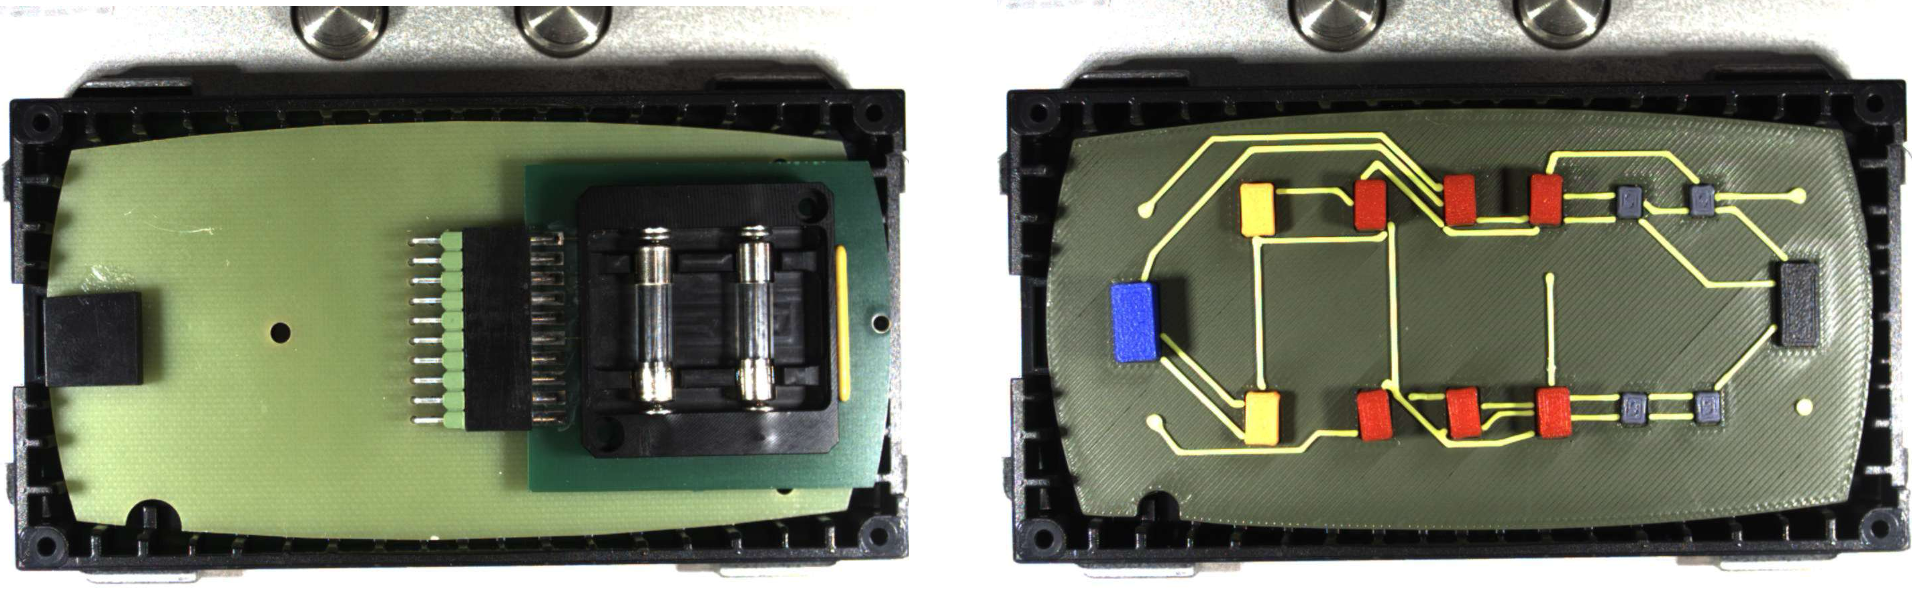
\includegraphics[width=1\textwidth]{PCBs.png}
    \caption{Gegenüberstellung der alten und neuen \ac{PCB}s}
    \label{fig:PCBs}
\end{figure}

Wie auch auf der \autoref{fig:PCBs} zu sehen ist, bieten die neuen PCBs weit mehr Details und sind daher komplexer als die \ac{PCB}s, die für die Machbarkeitsstudie verwendet wurden. 
Dies führt zu mehr Möglichkeiten, die Möglichkeiten des Modells zu testen und die Klassifikation zu verbessern. Die Reevaluierung des Modells mit den neuen Daten wird in \autoref{sec:reevaluierung} beschrieben.

